\section*{Research Design}

The empirical analysis presented below uses the country-year as the unit of analysis, covering years from 2002 (when the ICC became active) through December 2016.  While we would prefer to limit our sample to cases with some minimal expectation of ICC involvement, identifying that set of `at-risk' cases is nontrivial. One possibility would be to establish as the relevant population of cases only those situations that have been referred to the Court by communications from states, international organizations, and non-governmental organizations. The Court, however, has not made details on communications received publicly available, and numerous attempts to obtain this information have gone unanswered. Another possibility would be to restrict the sample of potential cases to countries with high levels of one-sided violence, human rights violations, etc. However, these factors that likely influence the expectation of ICC involvement are included in our models as independent variables, precluding us from using them to select our cases. We therefore use all country-years as our sample for analysis. This allows us to investigate potential ICC involvement in all states since 2002 without relying on potential explanatory variables to select a relevant set of observations.\footnote{As a robustness check, we do limit our sample when modeling ICC involvement to a restricted set of cases that (1) have experienced a political terror (PTS) score of 3 or higher or (2) have experienced civil conflict at some time since 2002. Restricting the sample in this way does not significantly change our key empirical results.}

%note: we might want to FN most of this discussion -- it seems weird to start our research design section by addressing issues our analysis. of ocuse, we also need to discuss # of countries, observations, etc. here. 

\emph{Response Variables}

The empirical analysis below tests the determinants of moving from no ICC involvement, to a preliminary investigation, and then to a formal investigation; while also accounting for the target of the ICC's involvement. Specifically, we examine two sequentially ordered dependent variables: 

% note from sm: better labeling
\begin{itemize}
	\item State-Focused ICC Transition
	\item Opposition-Focused ICC transition
\end{itemize}

To measure these variables, we first need to determine what constitutes involvement in a particular country by the ICC. To do this, we first identify whether the behavior of, or actions taken by, officials or nationals of a particular country is explicitly being examined or investigated by the ICC. Evidence of this includes explicit references to the behavior of or crimes potentially committed by nationals of that country in ICC reports and documentation. We examined a variety of documents from the ICC, including press releases on the opening of examinations/investigations, yearly reports on the Court's activities, summary reports for ongoing cases, etc. Importantly, this coding rule means that the state associated with a particular ``situation'' is not necessarily the state, or the only state, experiencing ICC involvement. For example, the situation referred to the ICC by Comoros, Greece, and Cambodia does not involve an investigation of actions taken by these states or their nationals, but instead is focused on potential abuses committed by Israel. We therefore treat Israel as the target of ICC involvement, while excluding Comoros, Greece, and Cambodia as ICC targets. Additionally, in the court's preliminary examination focused on Afghanistan, both Afghanistan and the United States are implicated. This is because reports provided by the ICC on it's preliminary examination activities explicitly refer to potential abuses perpetrated by Afghan forces and nationals, as well as to potential abuses committed by US forces in Afghanistan. Thus, ICC involvement is coded for both Afghanistan and the United States.

After identifying which states have experienced ICC involvement, we then develop a scheme to code the transition from no ICC involvement to the onset of a preliminary investigation. \emph{State-Focused ICC Transition} is coded 1 in the year the ICC begins a preliminary examination in which the government is targeted. We consider the ICC's actions to be government-targeting if they involve examining/investigating actions taken by current members of the state's security forces or current political leaders. We also consider actions to be state-targeting if the Court investigates alleged crimes committed by supporters of or groups supported by the current regime.\footnote{For example, this includes crimes allegedly committed on behalf of Kenyan government officials by private citizens (i.e. lawyers engaging in witness tampering on their behalf). This would also include crimes allegedly committed by pro-government militia groups that receive state backing.} This variable is coded 0 in all other years. This variable is coded 1 in 90 of 2,906 observations (3\%). \emph{Opposition-Focused ICC Transition} is coded 1 in the year the ICC begins a preliminary examination targeting opponents of the state in question. Opponents include current rebels, political opponents, and any others who are not considered state targets. This variable is coded 0 in all other years. This variable is coded 1 in 66 of 2,906 observations (2\%).\footnote{In several cases, both state and opposition figures are implicated in the ICC's actions. In these cases, both transitions variables are coded 1.}

Next, we account for whether the ICC investigation moved from a preliminary to a formal investigation. We code \emph{State-Focused ICC Transition} and \emph{Opposition-Focused ICC Transition} as a 2 in the year that a formal investigation commences. Thus \emph{State- and Opposition-Focused ICC Transition}, measure the level of ICC involvement in a given year on a scale from 0 to 2. For both variables, we code the highest level of ICC involvement reached in any given year that is focused on a current member or supporter of the government (state-focused) or opposition (opposition-focused). The levels of ICC involvement are as follows: 0 if there is no ICC involvement, a 1 is coded if the highest level of ICC involvement in the current year is a preliminary examination. This includes referrals from states parties or the UN Security Council that have not yet progressed to a formal investigation. A 2 is coded for country months in which a formal investigation is ongoing (the latter category includes cases that have progressed to the stage of outstanding warrants or summons and ongoing trials).\footnote{We do not distinguish between stages after a formal investigation because of the small number of cases that actually advance to that point.}
% , but which have not progressed to the issuing of warrants or beyond. A 3 is coded for country months in which the highest level of ICC activity is an outstanding warrant or summons (i.e. that warrant/summons has not been executed). A 4 is coded for country months in which the highest level of ICC activity involves a suspect being in custody at the Hague and/or hearings ongoing to determine whether or not to confirm charges against a suspect. A 5 is coded once charges have been confirmed against a suspect, but before a trial begins, and a 6 is coded if a trial is ongoing.\footnote{Ongoing trial involves everything from the opening of the trial through the sentencing phase.}

It is also important to note that these variables are coded based upon the status of those being investigated in any given year. This means that the highest level of state or opposition-focused ICC involvement may change if those under investigation switch sides. This can occur, for example, if a regime change occurs in which targeted government officials lose power or targeted opposition members come to power.

One brief example will help elucidate the coding of these variables. First, the ICC initiated a preliminary examination into the situation in Colombia in 2004. The Court's examination explicitly focuses on actions taken both by rebel organizations opposed to the state (i.e. FARC and ELN) and pro-government paramilitaries and the state's own security forces. The ICC's examination, furthermore, has not proceeded to the formal investigation stage. Therefore, \emph{State-Focused ICC Transition} is coded 1 from 2004 through 2015, as there is an ongoing preliminary examination during this time that potentially implicates state officials. \emph{Rebel-Focused ICC Escalation} is also coded 1 from 2004 through 2015, due to the ongoing preliminary examination that implicates members of opposition groups.

% note from sm: probably not the best case to highlight since all the action in the dv happens in a one year period and all we see is a transition from 0 in 2010 to 2 in 2011 to 0 in 2012
% Second, the ICC has been involved in the situation in Libya since February 2011, when it was referred to the OTP by the UNSC. By March, the ICC's involvement progressed to a formal investigation, and by June 2011, warrants were issued. Those warrants remain outstanding today. At the beginning of the ICC's involvement, the Court's efforts were focused on current state officials -\/- Gaddafi and members of his inner circle -- and therefore the ICC's involvement is coded as State-focused. This changed, however, in September 2011, when the Gaddafi regime fell and former regime opponents took power. As a result, our coding changes in September 2011, such that Opposition-Focused ICC Involvement is coded 3 from that month on.

Based upon the above coding rules, \emph{State-Focused ICC Transition} has the following distribution: 0) 2,786 observations 1) 90 observations, and 2) 30 observations. \emph{Rebel-Focused ICC Escalation} is distributed as follows: 0) 2,775 observations 1) 66 observations, and 2) 65 observations.

\begin{figure}
    \centering
    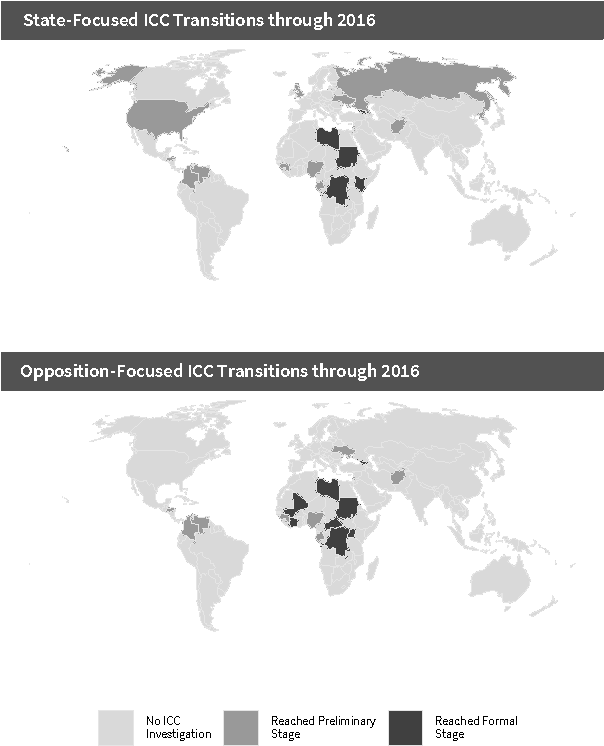
\includegraphics[width=1\textwidth]{iccMaps.pdf}
    \caption{Caption}
    \label{fig:iccMaps}
\end{figure}
\FloatBarrier

\emph{Legal Mandate Variables }

The legal mandate argument suggests that the OTP will base its case selection on the gravity of abuses committed and/or jurisdictional issues. To test this expectation, we include variables that account for violations of international humanitarian law. First, civilian targeting provides a useful metric for identifying human rights abuses committed by state and opposition officials because the extrajudicial killing of noncombatants is expressly prohibited by international humanitarian law (Blank and Noone 2013).

We use the Uppsala Conflict Data Program's (UCDP) Georeferenced Event Dataset (GED) version 5.0 to identify the number of civilians killed by government and opposition groups in any given month (Melander and Sundberg 2013). The GED is an events dataset that includes information on all instances of civilian targeting, or One Sided Violence (OSV), perpetrated by governments and nongovernmental actors between 1989 and 2015. These data have several advantages over other measures of human rights violations. First, they are available through 2015, whereas many other existing datasets that capture human rights practices end earlier, which would force us to shorten our analysis timeframe and ignore important cases of ICC involvement. Second, these data allow us to identify the perpetrators of human rights violations. Other possible datasets such as PTS and CIRI provide only a single country-level `score', which identifies the level of human rights violations in a given country. They do not allow us to identify violations perpetrated by non-state actors, as the scores generally refer to state-based abuses. This is critically important, given that ICC action is often directed at specific non-state or opposition actors within the state, not at the state itself. Measuring violations of human rights perpetrated only by the state, therefore, is insufficient as a predictor of directed ICC involvement. Finally, the OSV data provided by GED provides several advantages over other measures because it is events-level data. It can therefore be easily aggregated to generate a measure of the magnitude of OSV perpetrated by government or non-state actors in a given year. %Other Human Rights datasets, which provide a yearly summary measure of human rights violations, provide less variation and are not as compatible with our monthly data on ICC involvement.

To measure government OSV, we first generate the sum of all civilians killed in one-sided violence events perpetrated by each government in a particular year based upon the raw events data from GED.\footnote{The GED does not include data for Syria, but otherwise has global coverage. We therefore include data from UCDP's One-Sided Violence dataset (Eck and Hultman 2007) for Syria. While this is an imperfect solution, it does allow us to include Syria, a potentially important case, in our analysis. It is also better than using some other data sources that have more micro-level civilian deaths data, as the definition of OSV is not the same across other data sources, whereas the two UCDP dataset use the same definition of civilian targeting. Finally, it is important to note that our results remain consistent if we exclude Syria from the analysis.} We then generate a running sum of the number of civilians killed in government-perpetrated OSV since 2002 through the current year. This running sum provides a measure of the magnitude of human rights violations perpetrated by the state since the ICC became active. It is important to use this running sum rather than a simple measure of deaths in a given year because the Court can decide to investigate instances of war crimes or crimes against humanity that occurred any time since a state came under its jurisdiction or since the court became active (if referred by the UNSC or the state itself).\footnote{An alternative would be to create a running sum of OSV perpetrated since the state became a ratifier of the Rome Statute. However, this would not allow us to include states that have not ratified the Rome Statute, and would ignore the fact that states can come under investigation by the ICC for crimes committed despite non-ratification if they are referred by the UNSC or a non-state party who accepts the Court's jurisdiction on an ad hoc basis.} In our model predicting State-Focused ICC Onset, we therefore include the natural log of the running sum of state-perpetrated OSV since 2002. Last, we allow the affect of this variable to vary between the no investigation to preliminary stage and preliminary and formal stages. We do this to distinguish the effect this variable will have on just the onset of an investigation and the transition to a formal investigation. 

% In our model predicting State-Focused ICC Escalation, we measure the level of government-perpetrated OSV that occurred during the period under examination/investigation. For each preliminary examination and investigation, the ICC reports, often with great specificity, a particular date range that constitutes the focus of its inquiry. For example, The ICC's investigation of the situation in Georgia explicitly focuses on the events of July 1 through October 10, 2008. Some investigations are more open-ended; for example, the investigation in Uganda focuses on events since July 1, 2002, inclusive of today. This variable, therefore, identifies the period under investigation and then sums the total government-perpetrated OSV committed during that period. If the period of investigation is ongoing (e.g. Uganda) in the current month, this variable equals the running sum since the start of the period under investigation, through the current month. This variable is logged to account for its skewed distribution. The variable ranges from 0 to 8.6 with an average of 3.6.

In our models predicting \emph{Rebel-Focused ICC Escalation}, we create an analogous variable to that created for the state. We start by identifying all OSV perpetrated by non-state actors on the territory of a given state in a given year. We then sum those deaths to create a monthly total number of civilians killed by non-state actors in a given state in a given year. In the onset equation, we include the natural log of the running sum of opposition-perpetrated OSV since July 2002. This variable ranges from 0 to 9.3 with an average of 4.9. In the escalation equation, we include the total non-state perpetrated OSV committed during the period under investigation, or, if the period of investigation is ongoing, from the start of the period of investigation through the current year. 

%note: we probably have to justify using Vdem's lower court variable instead of higher court one, and acknoweldge that this measure is an imperfect proxy for complementarity.

Finally, we include a measure of lower court judicial independence from the Varieties of Democracy (V-Dem) project Lindberg et al. (2014). Higher values of this measure indicate greater independence of a state's judiciary.\footnote{The specific question asked in the V-Dem survey is: ``When judges not on the high court are ruling in cases that are salient to the government, how often would you say that their decisions merely reflect government wishes regardless of their sincere view of the legal record?''. The surveys asks this question of respondents on an ordinal scale (0-4) and then combines responses using a measurement model.} This corresponds well with the principle of complementarity, as it proxies the willingness and ability of the judiciary to investigate alleged perpetrators of war crimes and crimes against humanity. States with strong, independent judiciaries have the capacity to investigate perpetrators, while those with weak, non-independent judiciaries cannot credibly threaten an independent, effective investigation. This holds for investigations that target both the state and opposition: a non-independent judiciary will be unable to hold state officials accountable because the judiciary is dependent upon those state officials. A weak judiciary, furthermore, will likely be unable to carry out an effective, unbiased investigation of opposition perpetrators. States with strong judiciaries, therefore, make both state-focused and opposition-focused ICC involvement unnecessary. We also model this variable to have differential effect on the transition between stages of the ICC process. %As discussed above, this effect should be particularly pronounced in the analysis of ICC escalation, as preliminary examinations may take place in states with strong judiciaries, but those examinations are unlikely to progress. 

\emph{Realist/Institutional Constraints Variables}

As argued above, it is likely that the Court considers the reactions of third party states, especially the P5, when it becomes involved in a situation. The implication is that the ICC might be more reluctant to target states that have strong ties with the P5. Based on this logic, we include several variables in our empirical analysis to account for a state's relationship with the P5.

%note: we should remind readers why we use P5 instead of a general list of major powers or whatever. 

% First, we include measures of military closeness to the P5. We create two dummy variables to identify ongoing military intervention by a P5 state into a given country. We collected original data on P5 interventions, as existing datasets either were unavailable for the time period covered in our investigation, or restricted their coverage to large interventions or only those during events such as civil wars (Koch and Sullivan 2010; Pickering and Kisangani 2009). To collect this information, we had coders search Lexis Nexis for news articles about military actions taken by each of the P5 states between 2002 and 2015. Excluded from this measure are military deployments that were humanitarian in nature, peacekeeping, or interventions intended to simply remove nationals of a P5 state from a risky situation. The variables we use in the analysis identify whether there is an ongoing military intervention by any P5 state in a given country-month. We also identify whether that intervention is pro-government or pro-opposition, which generates two dummy variables. The first, \emph{Pro-State Intervention} is coded one if there is an ongoing P5 military presence supporting the government in a given country-month. The second, \emph{Pro-Opposition Intervention,} is coded 1 if there is an ongoing P5 military presence supporting opponents of the current government in a given country-month. Pro-State Intervention is coded 1 in 974 of 31,175 observations, while Pro-Opposition Intervention is coded 1 in 695 of 31,175 observations.

% We also include a measure of alliance commitments between the state in question and the P5. This variable, which is coded 1 if the state in question has a defensive pact with any P5 member in the current year, is used as a second measure to capture the military closeness of a given state to any P5 member. We focus on defensive alliances because these represent the highest level of military commitment, suggesting that the state is important to the P5 state. The advantage of this variable is that while a military intervention may be better at capturing the immediate links between the state and a P5 member, there may be no need for military intervention in a given month. Alliance commitments, which are more long-term, should pick up on the underlying military closeness of the state with the P5 in situations where there is no active military intervention. We use the Correlates of War data on military alliances to code this variable (Gibler 2009).\footnote{We are unable to use the Alliance Treaty Obligations and Provisions (ATOP) data because it ends in 2003.} It is coded 1 in 10,296 observations. It is lagged 1 year in the analysis.

To measure P5 closeness, we include a measure of the minimum ideal point distance from the given state to the closest P5 state. This measure is lagged 1 year. The ideal point data come from Bailey et al. (Forthcoming). Our expectation is that as this minimum distance increases, the state in question gets farther and farther from the P5 in terms of policy similarity. This suggests that the P5 have less of a vested interest in the government of that state, and ICC involvement should be more likely, as it will not threaten strong P5 interests. We expect this variable to have the opposite effect on ICC involvement focused on the opposition: as ideal point distance to the closest P5 member increases, the P5 are more likely to have close ties with opposition groups in these dissimilar states, and will therefore have incentives to pressure the Court not to get involved in an opposition-focused examination or investigation. 

\emph{Control Variables }

We also include several control variables to account for alternative explanations of ICC involvement. First, we include a binary variable to account for whether the state is in Africa. This variable equals 1 if the country is on the African continent, and zero otherwise. As we suggest throughout this paper, many commentators argue that the ICC has an Africa bias, as it has only initiated formal investigations in African nations. We thus expect that the ICC will become more involved in situations in Africa.\footnote{In our model, we differentiate the effect that this variable has on the transition from no investigation to preliminary and preliminary to formal.} Second, we include a control for whether the state in question ratified the Rome Statute. Ratifying the Rome Statute is important because it gives the ICC jurisdiction over the state in question.\footnote{Ratification is not a prerequisite for ICC involvement, however, as the Security Council can refer situations in non-state parties (e.g. Sudan), and states can accept the Court's jurisdiction on a more limited basis (i.e. relating to a specific situation) without ratifying the Rome Statute.} The variable is binary; it equals 1 if the state ratified the Rome Statute and zero otherwise. Data were obtained from the ICC website.\footnote{\url{http://www.icc-cpi.int/EN\_Menus/icc/Pages/default.aspx}} We also include polity as a measure of regime-type (Marshall and Jaggers 2010). We expect the ICC to be less likely to become involved in situations in wealthier and more democratic states, as these states likely have the resources and willingness to address human rights violations domestically. Finally, we include a dummy variable to account for whether there is an ongoing civil conflicts in the state using the UCDP Armed Conflict Data (Themnér and Wallensteen 2012). We expect the ICC to be more likely to become involved if a civil war is ongoing. While the ICC is not responsible for prosecuting conflict per say, it is likely that the prevalence of conflict is correlated with war crimes. This variable is lagged one year.
